\chapter{Background}

\section{History of machine translation}

\XXX{is it ok to quote the whole paragraph with short history? e.g. \cite{Han2016}}

\section{Transformer model}

Introduced in \perscite{vaswani-2017-transformer} Transformer model is used as a base
for numerous state-of-the-art systems as can be seen for example in 
WMT18 \parcite{bojar-etal-2018-findings} and
WMT19 \parcite{barrault-EtAl:2019:WMT} results.

Prior to invention of the \textit{Transformer} model, RNN's and CNN's were used
to encode source side of the sentence pair and to decode it into the target sentence.
Various window lengths in CNN architectures allowed to capture long range relations
as well as short range ones; still the range was limited by the maximum window length.
In RNN-like architectures LSTM and GRU cells were used, as their structure allowed to
pass the internal state on longer distances due to selective forgetting.

\textit{Transformer} model uses \textit{self attention} mechanism to encode contextual
information in each word position. \textit{Position encoding} allows passing the position
information without explisit sequential connections as in RNNs.
As was stated by \textit{Transformer}'s authors, there are three main points why
self-attention mechanism should be preferred:
\begin{itemize}
  \item total computational complexity per layer;
  \item the amount of computation that can be parallelized;
  \item the path length between long-range dependencies in the network.
\end{itemize}

\begin{table}
\centering
\begin{tabular}{l|ccc}
\toprule
Layer type        &   Complexity             &  Sequential & Maximum        \\
                  &   per layer              &  operations & path length    \\
\midrule
Self-Attention    & $O(n^2 \cdot d)$         & $O(1)$      & $O(1)$         \\
Recurrent         & $O(n \cdot d^2)$         & $O(n)$      & $O(n)$         \\
Convolutional     & $O(k \cdot n \cdot d^2)$ & $O(1)$      & $O(log_k (n))$ \\
Self-Attention (restricted) & $O(r \cdot n \cdot d)$       & $O(1)$ & $O(n/r)$  \\
\bottomrule
\end{tabular}
\mycaption{Maximum path lengths, per-layer complexity and minimum number of sequential operations for different layer types} {
	n is the sequence length, 
	d is the representation dimension, 
	k is the kernel size of convolutions and 
	r the size of the neighborhood in restricted self-attention.
}
\label{tab:layer_complexity_comp}
\end{table}


\begin{figure}[h]
	\centering
	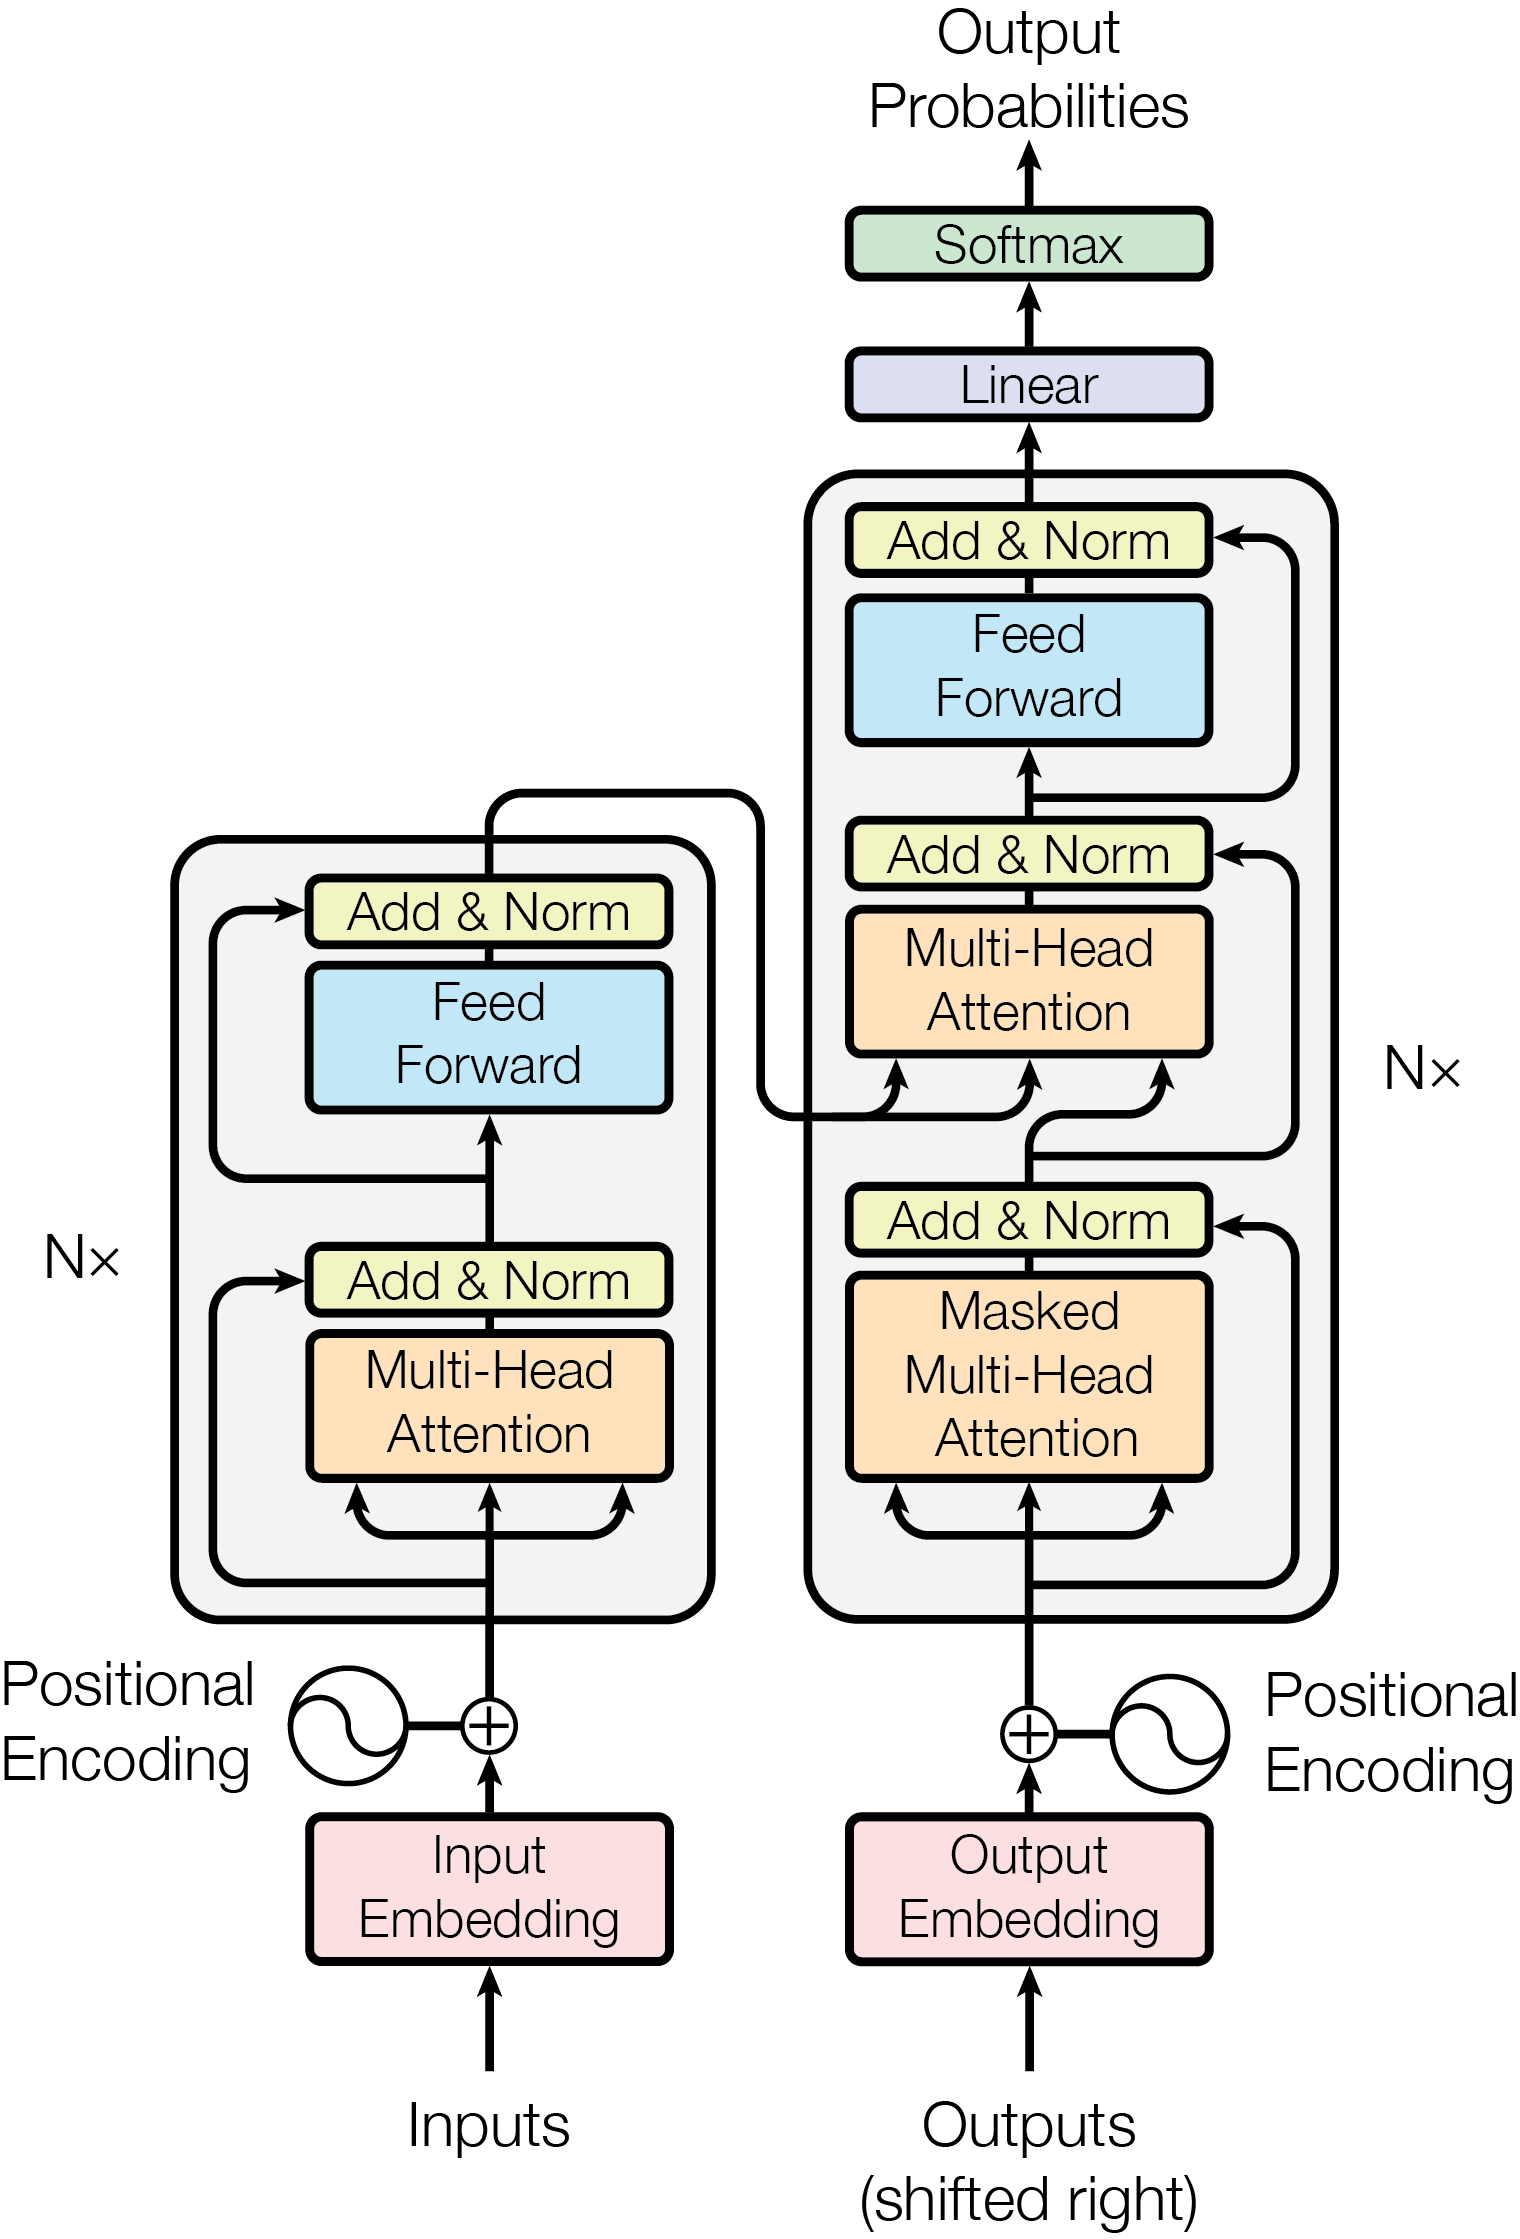
\includegraphics[width=0.9\columnwidth]{../img/transformer_architecture.png}
	\mycaption{Transformer model architecture} {}
	\label{fig:transformer_architecture}
\end{figure}

\section{Translation evaluation}

\subsection*{History}

In 1966 first machine translation evaluation methods were proposed
by the automatic language processing advisory committee (ALPAC).
The proposed metrics were "intelligibility" and "fidelity"\citep[p~67]{Translation1966}.
Metrics were considered independent and the evaluation was meant to be conducted
by two independent groups of raters.
\textit{Intelligibility} was measured without reference to the original by
group of raters fluent in target language and not familiar with the source language.
The raters were comparing the "informativeness" of evaluated translation with carefully
prepared reference translation. The metric scale was from 1 (hopelessly unintelligible)
to 9 (perfectly clear and intelligible).
\textit{Fidelity} to the sense of the original text was measured by another group of raters,
which were native speakers of the target language and highly proficient in the source language.
It was measured on a scale of 0-9 and showed how much additional information was added in
the evaluated translation comparing to the reference translation.

Advanced Research Projects Agency (ARPA)
\todo{from White 1999 and Church 1993}
comprehension evaluation, quality panel evaluation, and evaluation based on adequacy and fluency

Automatic evaluation

- Metric should correlate with human judgments;

- Works with texts of different domains

- Banerjee et al. (2005) correlation, sensitivity, consistency, reliability and generality.

\subsection*{BLEU - bilingual evaluation understudy}

In \cite{Papineni02bleu} was introduced a nowel method of audomatic machine translation evaluation -
BLEU (bilingual evaluation understudy). Its advantages are high speed and low cost of evaluation,
language independence and high correlation with judgements of highly skilled human raters evaluations.

Shortly, BLEU score incorporates modified n-gram precision scores corrected by brevity penalty,
which ensures the produced translation lenght is close to the reference one.
BLEU score is computed for the whole test corpus.

\subsubsection*{Modified \textit{n}-gram precision score}

The main element of the metric is the \textit{precision} measure.
To compute precision, the number of candidation translatin words (unigrams) that are present in
any reference translation is divided by the total number of words in the candidate translation.
This approach leads to overrating candidate translation which consist of only one or couple of
words that occur in reference translations, as can be seen in the expample below.

Intuitively, after a word from the reference translation has occured it should not be considered
in the calculation anymore. This intuition is formalized as the \textit{modified unigram precision}.
It is computed in the following way: first, the maximum number of occurances of a word in any
reference translation is counted; then the total count of every candidate word is replaced by the
maximum reference count, added up and divided by the initial total number of candidate words.
As a result, the sentence which may receive high precision score will receive more realistic evaluation
measured by modified precision score, as can be seen in the example below.\\

Candidate: \underline{of} \underline{of} \underline{of} of of of of of of of

Reference: London is the capital \underline{of} England and \underline{of} the United Kingdom
\underline{of} Great Britain and Northern Ireland.

Precision: 1

Modified unigram precision: 3/10
\\
Similarly is computed modified \textit{n}-gram precision score for any \textit{n}, but \textit{n}-gram
counts are collected instead.

\subsubsection*{Sentence length}

\subsubsection*{The formula}


\section{Multi-target machine translation}
\label{section:multitarget_mt}

\todo{move here parts of ch.3}
